\label{chap:main_work}
In this chapter, the main contents of the thesis work are represented.
Figure \ref{fig:framework} shows the framework of the memory power
optimization process using the simulated annealing algorithm.
There are two kinds of input for the simulated annealing algorithm.
One is the input data related to the optimization problem.
These raw data is recorded in different text files but their data
structure is not suitable for the simulate annealing algorithm.
Thus, a proper input data organization is defined and a parsing
method is used to transform the raw data into this data organization.
Section \ref{sec:input_organ} discusses the input data organization
and the parsing method in detail.
The other kind of input for the algorithm is the algorithm parameter.
The discussion of these parameters are made in Section.....which also
introduce the design of the simulated in detail.
\begin{figure}[H]
	\begin{center}
		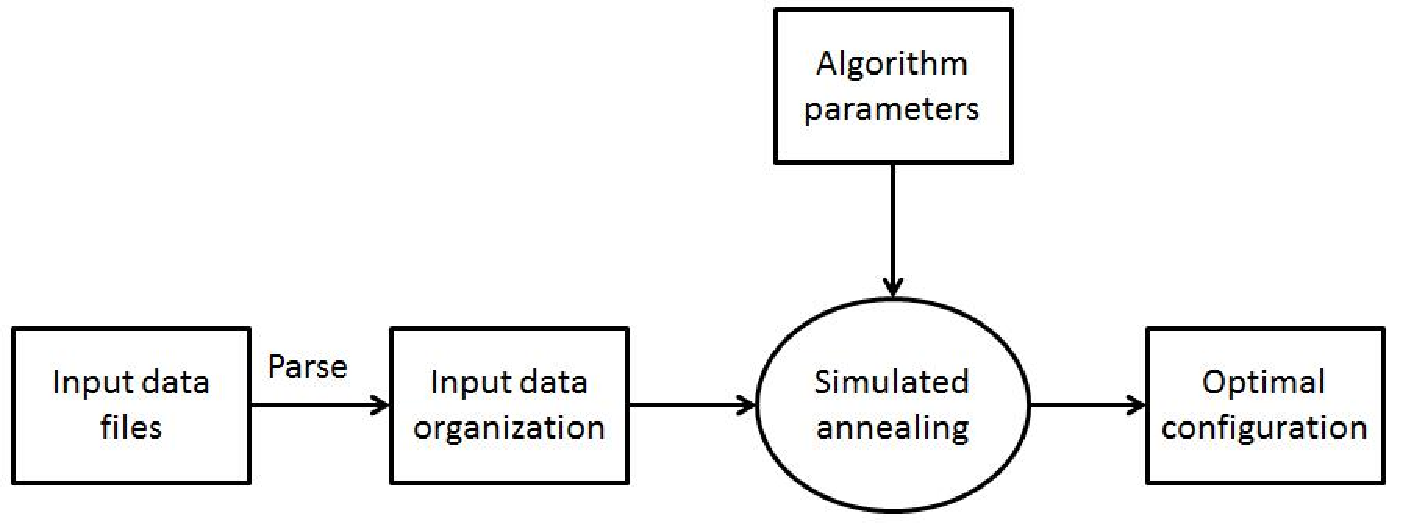
\includegraphics[width=0.7\textwidth]{optim_framework}
		\caption{Framework of The Simulated Annealing for Memory Power Optimization}
		\label{fig:framework}
	\end{center}
\end{figure}
	\section{Input data organization}
	\label{sec:input_organ}
	As discussed in Section \ref{sec:memory_partition}, the formal
	power model requires the parameters that are relevant to the
	memory types, the application profiles and the interconnect.
	Thus, these parameters are the input data to the simulated
	annealing algorithm.
	Since the object oriented programming is planned to be used for
	the implementation of the simulated annealing, the parameters
	that are related to the same item can be grouped together into
	one class. For example, the physical parameters that are
	relevant to the memory type can reside in the memory class.
	Figure \ref{fig:uml} shows the input parameters
	organization in the form of the UML class diagram.

	\begin{figure}[htb]
		\begin{center}
			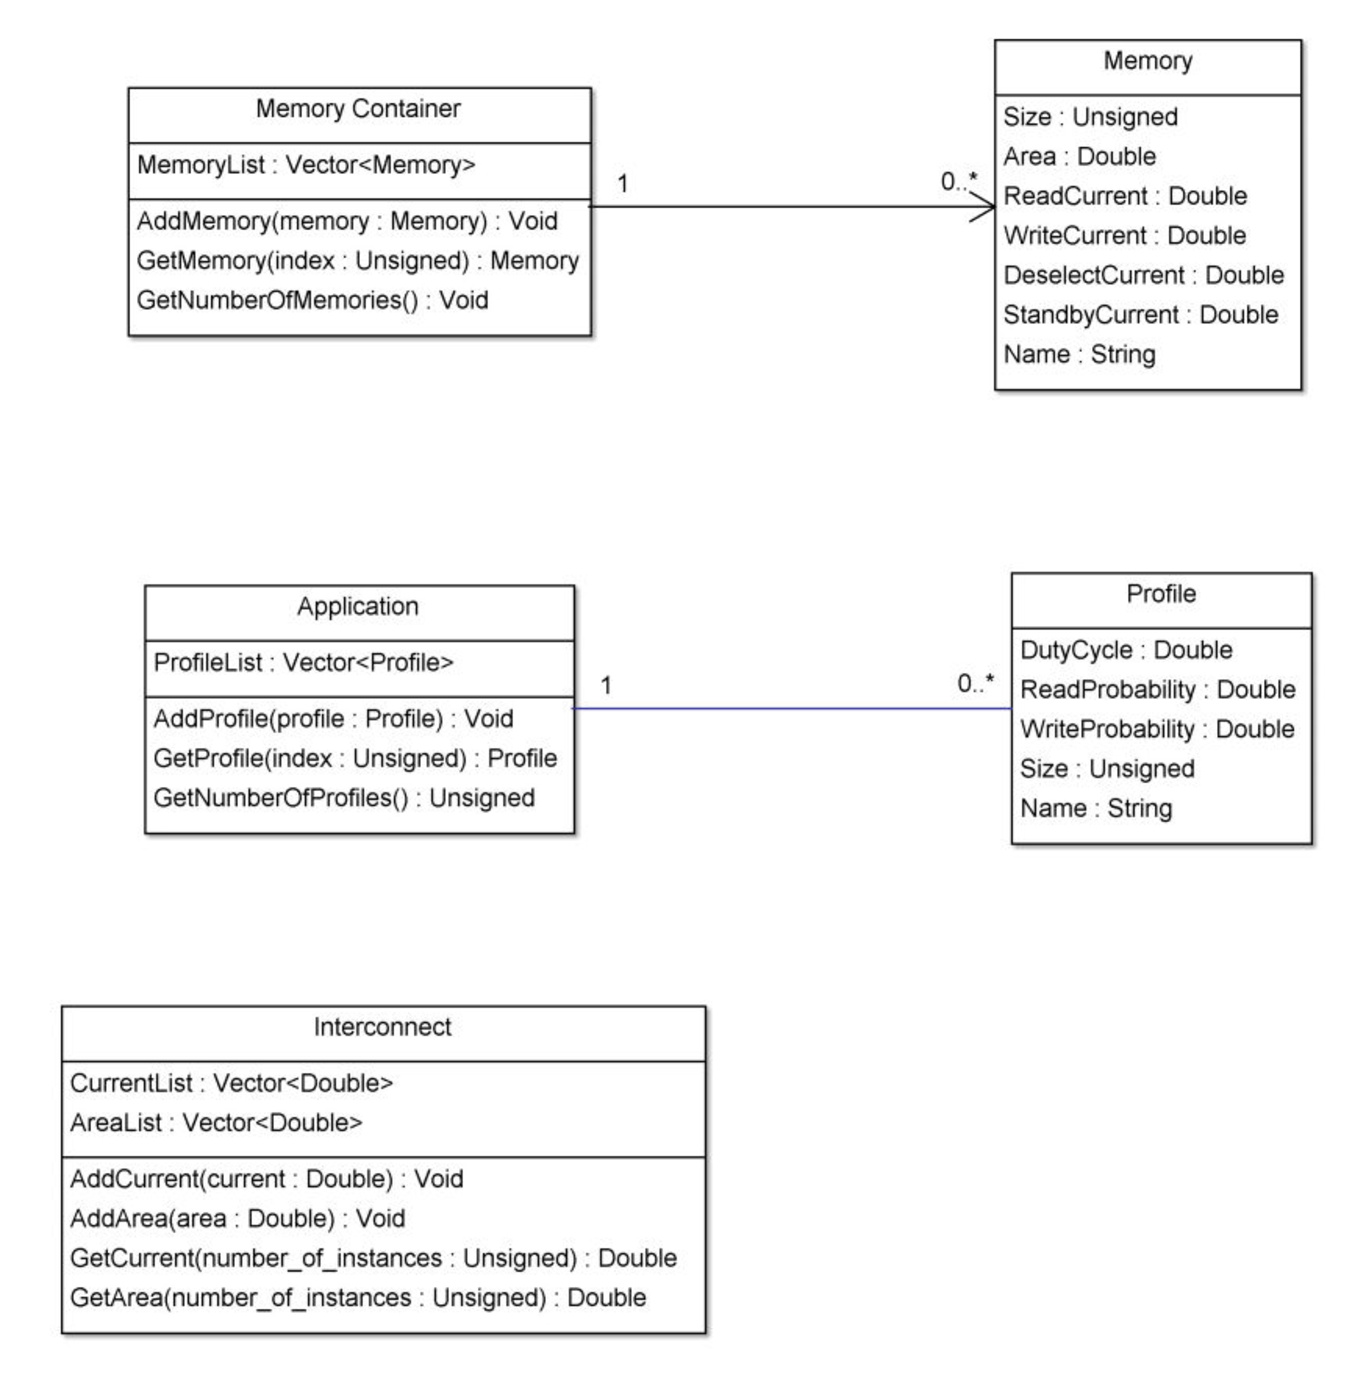
\includegraphics[width=0.7\textwidth]{uml_class}
			\caption{Input Parameter Organization in UML Diagram}
			\label{fig:uml}
		\end{center}
	\end{figure}
	
	The memory class includes all its parameters that are used in the
	formal power model.  Since there are a set of memory types in the
	power model, a set of objects of the memory class will be created in
	the simulated annealing algorithm as well. Thus the memory container
	class is defined to store these memory objects.
	And the algorithm can also retrieve the required objects and the
	total number of memory objects through the corresponding operations
	in the memory container class.
	The profile class and the application class are defined similarly
	to the memory class and the memory container class respectively.
	However, the interconnect is different. It uses two lists to store the
	current and area parameters whose value are dependent on the total
	number of instances. These parameters can be also retrieved by the
	simulated annealing algorithm through the corresponding operations
	defined in the interconnect class.
	\begin{figure}[htb]
		\begin{center}
			\subfloat[][]
			{
				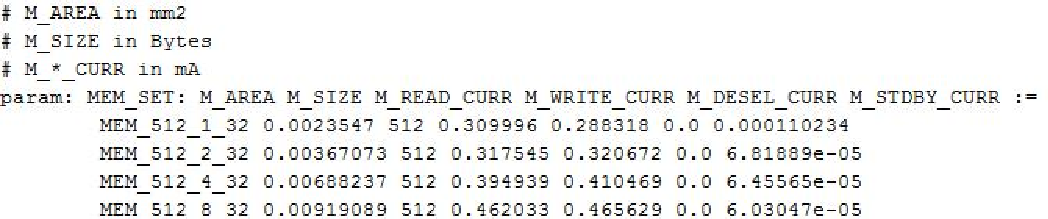
\includegraphics[width=0.7\textwidth]{mem_data}
				\label{subfig:mem_data}
			}
			\qquad
			\subfloat[][]
			{
				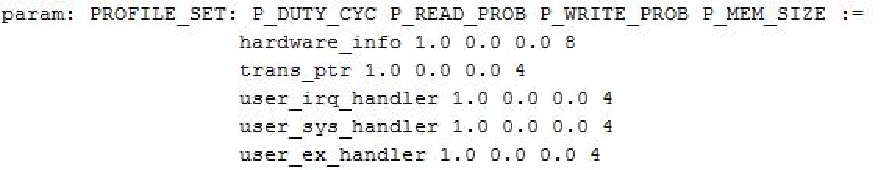
\includegraphics[width=0.7\textwidth]{profile_data}
				\label{subfig:profile_data}
			}
			\qquad
			\subfloat[][]
			{
				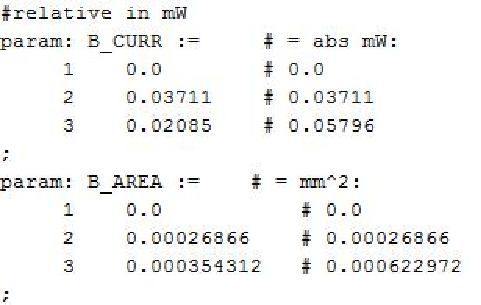
\includegraphics[width=0.4\textwidth]{ic_data}
				\label{subfig:ic_data}
			}
		\end{center}
		\caption{Fragments of The Input Parameter Data Files \cite{Strobel2016}}
		\label{fig;input_data}
	\end{figure}

	In this thesis work, the same data sets provided in \cite{Strobel2016}
	are used as the references for the input parameters data of the simulated
	annealing algorithm. These input parameters data are recorded in multiple
	plain text data files. Figure \ref{fig;input_data} represents some fragments
	of these data files. Figure \ref{subfig:mem_data} is the fragment of the
	memory data file. Figure \ref{subfig:profile_data} shows the fragment of the
	application profile data file and Figure \ref{subfig:ic_data} is the
	fragment of the interconnect data file. In order to group the data
	contained in these files into the designed input data organization, a
	parsing method is used. The basic idea of the parsing method is to read the
	plain text file line by line. The required data is extracted and the
	unnecessary data is discarded. Since the data file is text-based,
	the required data are converted into the corresponding data type during the
	extraction.

	\setlength{\textfloatsep}{0.2cm}
\begin{algorithm2e}[H]
	\KwIn{a memory\textbackslash profile data file, a memory container\textbackslash application object}
	\KwOut{void}
	\While{not end of the file}
	{
		read one line\;
		\If{relevant data is contaied in the line}
		{
			extract the data\;
			convert the extracted data into the corresponding type\;
			create a memory\textbackslash profile object based on the converted data\;
			add the created object into the list of the memroy container\textbackslash application object\;
		}
	}
	\caption{Parse Memory\textbackslash Profile Data File}
	\label{algo:mem_profile_parser}
\end{algorithm2e}
\setlength{\textfloatsep}{0.2cm}
	
	Algorithm \ref{algo:mem_profile_parser} is the pseudo-code of
	the parsing method for the memory and profile data files. If the method is
	used to parse the memory data file, it first reads one line of the file text.
	Then it checks whether there is the relevant data contained in the line or not.
	If there is no data, the the algorithm continues reading the next line.
	Otherwise, the relevant data is extracted and converted into the corresponding
	data type.
	It can be seen from the file fragment in Figure \ref{subfig:mem_data}, all the
	parameters data related to one memory type are listed in one single line.
	Thus, a memory object can be created based on the retrieved and converted data
	for one line. And the created object is added to the list in the memory container
	object. The same parsing step is repeated until the method reaches the end of
	the file. The parsing process of the application profile data file is similar
	to the parsing of the memory data file.
	The only differences are that it deals with the profile data file and the
	profile objects are created and added to the list of the application object.
	However, the parsing method of the interconnect data file is modified slightly.
	Algorithm \ref{algo:ic_parser} shows the pseudo-code of the parsing method for
	the interconnect data file.
	From the file fragment in Figure \ref{subfig:ic_data} it can be seen that there
	are two parts in the interconnect data file.
	The first part contains the interconnect current data while the other part
	records the interconnect area data. Thus, after the extracted data is converted,
	the parsing method needs to check whether the data is related to the current or
	the area. Then the data is added to the corresponding list of the interconnect
	object.
	
	\setlength{\textfloatsep}{0.2cm}
\begin{algorithm2e}[H]
	\KwIn{an interconnect data file, an interconnect object}
	\KwOut{void}
	\While{not end of the file}
	{
		read one line\;
		\If{relevant data is contaied in the line}
		{
			extract the data\;
			convert the extracted data into the corresponding type\;
			\eIf{is current data}
			{
				add the converted data into the current list of the interconnect object\;
			}
			{
				add the converted data into the area list in of interconnect object\;
			}
		}
	}
	\caption{Parse Interconnect Data File}
	\label{algo:ic_parser}
\end{algorithm2e}
\setlength{\textfloatsep}{0.2cm}
	
	\section{Simulated annealing design flow}
	\label{sec:sa_design_flow}
	The major design of the simulated annealing for the memory power optimization is
	the algorithm framework. Before the detail of the design concepts are introduced,
	an abstract design flow of the simulated annealing algorithm is provided in Figure
	\ref{fig:sa_framwork}. From the figure it can be seen that there are three major
	steps in the design flow. The first step is the initialization of the algorithm.
	The second step is the inner loop and the third step is the outer loop.
	To illustrate the algorithm design clearly, the design concepts that are discussed
	later in this chapter answer the following questions step by step:
	
	\begin{itemize}
		\item What is the solution $S$ and its representation?
		\item What is the solution neighborhood structure and its method $Neighbor()$ to
		generate the neighboring solution $S_{neigh}$ from the current solution $S_{curr}$.
		\item What is the objective function $Cost()$ to calculate the cost $C$ of the solutions?
		\item What is the procedure of the metropolis criterion $Metropolis()$?
		\item What is the cooling schedule $CoolingSchedule()$?
		\item What is the termination conditions for the inner loop $Termination_{inner}()$ and
		the outer loop $Termination_{outer}()$?
		\item How to determinate the initial solution $S_{0}$ and the initial temperature $T_{0}$?
	\end{itemize}

	\begin{figure}[htb]
		\begin{center}
			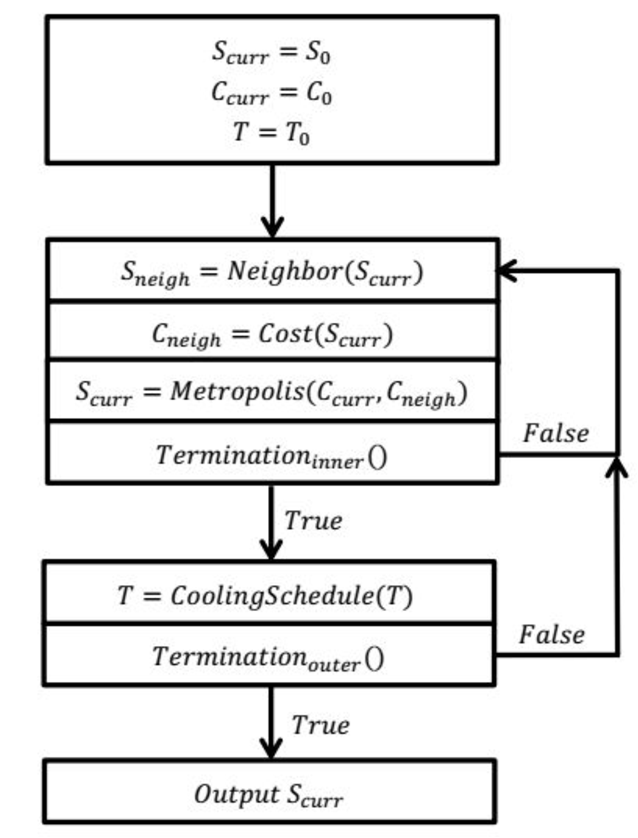
\includegraphics[width=0.7\textwidth]{sa_framework}
			\caption{Simulate Annealing Design Flow}
			\label{fig:sa_framwork}
		\end{center}
	\end{figure}

	\section{Stage 1}
	\label{sec:stage_1}
	As discussed in Section \ref{sec:memory_partition}, the result of the memory
	partitioning process is a configuration for memory system. The configuration
	is consisted of the allocation of the memory set and the binding of the
	application profiles. The solution provided by the simulated annealing
	algorithm should correspond to the memory configuration. According to this,
	the solution of the simulated annealing algorithm is defined as following.
	A solution is in the form of a integer vector that are divided into two parts.
	The first part of the vector corresponds to the allocation of the memories.
	Each element in this part is the number of the memory instances of the
	corresponding memory type. The second part of the vector contains the
	information about the binding of the application profiles. Each element
	in this part is the index of the memory type to which the corresponding
	profile is bound. Thus, the length of the vector is the sum of the number
	of the memory types and the number of the profiles.
	To be clear, the first part of the vector is called the allocation part of
	the solution while the second part of the vector is called the binding part
	of the solution. Figure \ref{fig:solu_exam_1} shows a solution example
	with two memory types and three application profiles. In the allocation part,
	one instance for both memory types is allocated. In the binding part, the
	profile 0 is bound to the memory type 0. The profile 1 and 2 are both bound
	to the memory type 1.
	\begin{figure}[t]
		\begin{center}
			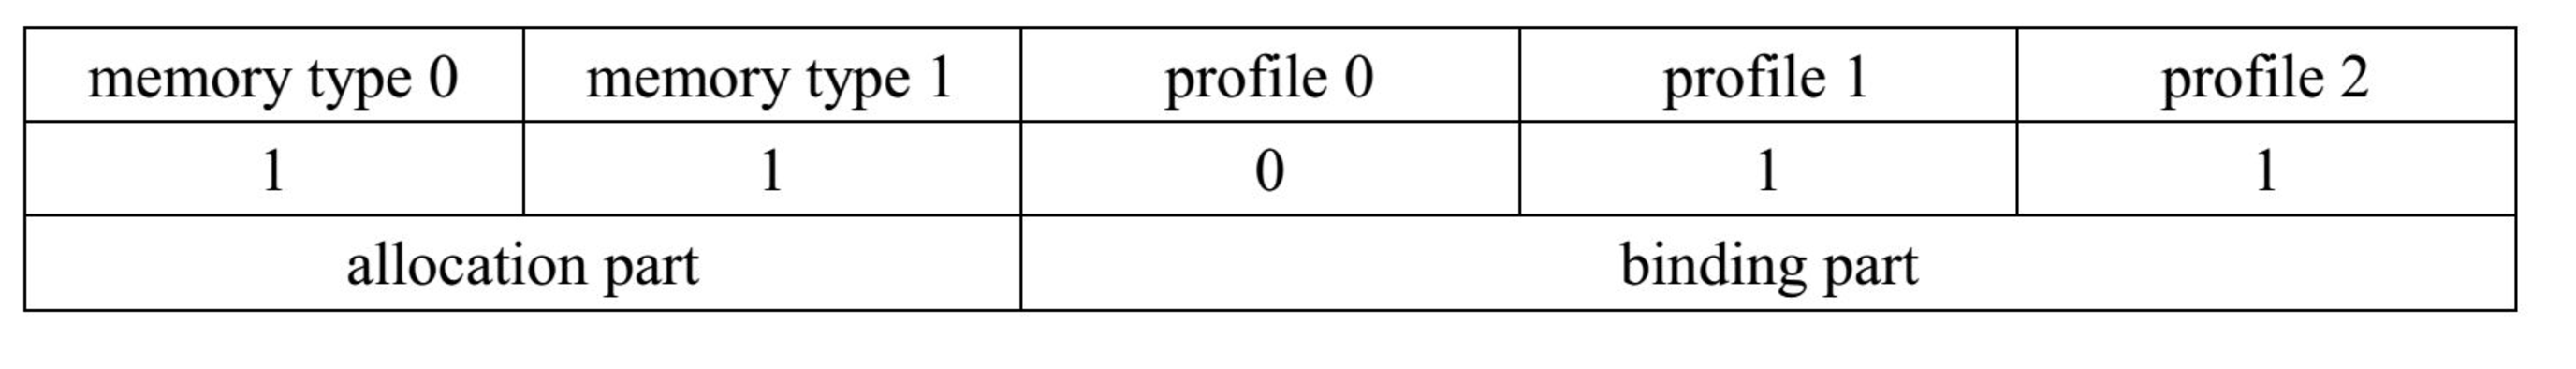
\includegraphics[width=0.7\textwidth]{solution_example_1}
			\caption{A Solution Example}
			\label{fig:solu_exam_1}
		\end{center}
	\end{figure}

	According to the solution definition, the neighborhood structure is described
	as following. A neighboring solution is a vector with same length of the
	original solution and only one element value in the vector is different from the
	original solution. Figure \ref{fig:neigh_solu_exam_1} shows an example of the
	neighboring solution. The original solution is the same in Figure
	\ref{fig:solu_exam_1}. In the neighboring solution 1, two memory instances are
	allocated for the memory type 0 while only one instance is allocated in
	the original solution. The rest part of the neighboring solution 1 are the
	same with the original solution. In the neighboring solution 2, the only
	difference to the original solution is that the profile 2 is bound to the
	memory type 0.
	\begin{figure}[b]
		\begin{center}
			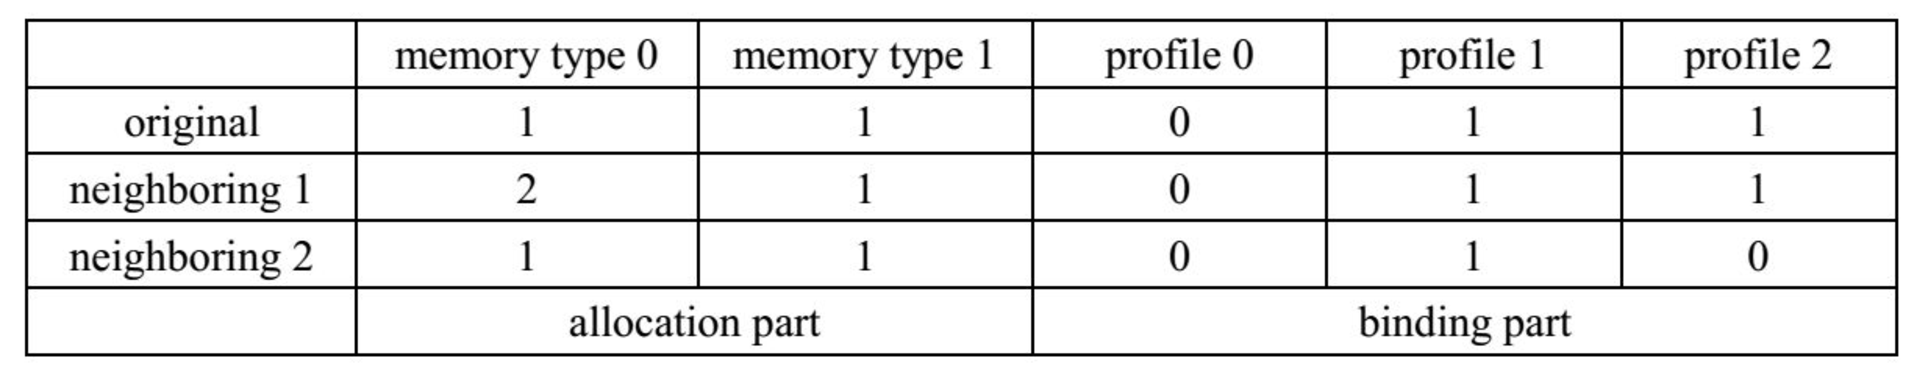
\includegraphics[width=0.7\textwidth]{neigh_example_1}
			\caption{Neighboring Solutions Example}
			\label{fig:neigh_solu_exam_1}
		\end{center}
	\end{figure}	
	In the simulated annealing algorithm, the neighboring solutions are generated by
	the method $Neighbor()$. The basic idea of generating neighboring solutions
	is to select one element from the current solution and modify the value of this
	chosen element.
	However, the constraints of the formal power model should be also taken into
	consideration in the design of the $Neighbor()$.
	For constraint 1, the total number of allocated instances can not be larger than
	the predefined limit $mems_{max}$. To satisfy this constraint, the new value for
	the modified element in the allocation part should be limited in a range.
	The lower bound of the range is 0. The upper bound the range is computed as following.
	Firstly, calculate the total number of memory instances $mems_{total}$ in the
	current solution. Suppose solution element $i$ in the allocation part is to be modified.
	Let $mem_{i}$ denotes the value of element $i$ in the current solution.
	Then the upper bound of the value range is $mems_{max}-mems_{total}+mem_{i}$.
	
	Because the solution of the simulated annealing algorithm corresponds to the
	memory configuration, the solution cost $C$ is defined as the average power
	consumption of the configuration. The object function $Cost()$ is designed
	based on the formal power model that is introduced in Section
	\ref{sec:memory_partition}. All the relevant parameter data required by the
	power model can be fetched from the input parameter organization.
	
	The procedure of the metropolis criterion is straightforward and it is
	illustrated in Algorithm \ref{algo:metropolis}. Because the goal of the
	power memory optimization is to reduce the power consumption, the solution
	with lower cost is considered as the better one in the metropolis criterion.
	A random real number $R$ is generated by a method $Random()$.
	This method only generates real numbers that are uniformly distributed in the
	range of 0 to 1 due to $R$ is compared with a probability $P_{accept}$.
	
	\setlength{\textfloatsep}{0.2cm}
\begin{algorithm2e}[h]
	\KwIn{$C_{curr},C_{neigh},T$}
	\KwOut{void}
	\eIf{$C_{curr} \leq C_{neigh}$}
	{
		$S_{curr}=S_{neigh}$\;
		$C_{curr}=C_{neigh}$\;
	}
	{
		$P_{accept}=\exp{\left( -\frac{C_{neigh}-C_{curr}}{T} \right)}$\;
		$R = Random()$\;
		\If{$R \leq P_{accept}$}
		{
			$S_{curr}=S_{neigh}$\;
			$C_{curr}=C_{neigh}$\;	
		}
	}
	\caption{Metropolis Criterion Precedure}
	\label{algo:metropolis}
\end{algorithm2e}
\setlength{\textfloatsep}{0.2cm}
	
	For the cooling schedule, the temperature $T$ is linearly reduced with a fixed
	cooling ration $R_{cool}$. Equation \ref{equa:cooling_sche} is the designed
	of the cooling schedule.
	Obviously, the value of the $R_{cool}$ should be
	a positive real number and it must be less than 1 in order to decrease the
	temperature. However, it is a non-trivial task to determine the proper value of
	the cooling ration. In this approach, the value of $R_{cool}$ is set to 0.85
	first and it can be adjusted base on experiments.
	\begin{equation}
	\label{equa:cooling_sche}
		T_{N+1}=R_{cool} \cdot T_{N}
	\end{equation}
	The initial solution $S_{0}$ of the simulated annealing algorithm can be set to a given
	solution manually. In this approach, the initial solution is set as following.
	Only one larger enough memory instance is allocated so that all the application
	profiles can be bound to it.
	For the determination of the initial temperature $T_{0}$, the initial acceptance
	probability $P_{0}$ is used. As S. Kirkpatrick et al. propose in the original article,
	$P_{0}$ is the expected acceptance probability of the worser solution at the initial temperature.
	In this approach, the value of $T_{0}$ is computed by Equation \ref{equa:t_0_1} based
	on the metropolis criterion. In the equation, $\left( C_{neigh}-C_{curr} \right)_{max}$
	is the maximum cost difference between a worser neighboring solution and the current
	solution. It can be measured by generating a set of worser neighboring solutions of the current solution randomly. The value of $P_{0}$ should be a positive real number
	less than 1. It is also should close to 1 because the neighboring solutions are randomly
	accepted at $T_{0}$. The value of $P_{0}$ is set to 0.85 in this approach and it can be
	adjusted based on experiments.
	\begin{equation}
	\label{equa:t_0_1}
		T_{0}= - \frac{\left( C_{neigh}-C_{curr} \right)_{max} }{ln{P_{0}}}
	\end{equation}	
	For the inner loop of the simulated annealing algorithm, the
	number of iterations is limited to a maximum number $Max_{iteration}$. During the
	execution of the inner loop, the number of iterations $Num_{iteration}$ is counted.
	When $Num_{iteration}$ becomes larger than $Max_{iteration}$, the inner
	loop terminates. The value of $Max_{iteration}$ is related to the size of the
	neighborhood structure $Size_{neighbor}$. Equation \ref{equa:iteration_innerloop}
	illustrates how to calculate the value of $Max_{iteration}$. From the equation it
	can be seen that $Max_{iteration}$ is proportional to $Size_{neighbor}$ with a
	factor $F_{iteration}$. The value of $F_{iteration}$ should be a positive real
	number. In this approach, it is set to be 1 and it can also be modified based on
	experiments.
	\begin{equation}
	\label{equa:iteration_innerloop}
		Max_{iteration}=F_{iteration} \cdot Size_{neighbor}
	\end{equation}
	For the outer loop termination, a low temperature limit $T_{low}$ is defined. When the
	temperature $T$ is decreased to $T_{low}$, the outer loop terminates. The determination of
	$T_{low}$ is similar to the determination of $T_{0}$. $P_{low}$ is defined as the expected
	acceptance probability at $T_{low}$. Then $T_{low}$ is computed according to
	\ref{equa:t_low_1}. In the equation, $\left( C_{neigh}-C_{curr} \right)_{min}$ is the
	minimum cost difference between a worser neighboring solution and the current
	solution. It is can be measured by generating a set of worser neighboring solutions randomly
	as well. The value of $P_{low}$ should be a positive real number close to 0 because the
	simulated annealing algorithm behaves like the local search algorithm at $T_{low}$. The
	worser neighboring solutions are seldom accepted. In this approach, the value of $P_{low}$
	is set to 0.1 and it can be adjusted base on experiments.
	\begin{equation}
	\label{equa:t_low_1}
		T_{low}= - \frac{\left( C_{neigh}-C_{curr} \right)_{min}}{ln{P_{low}}}
	\end{equation}	
	
	
	
	
	
	
	